\documentclass{article}
\usepackage[T1]{fontenc}
\usepackage[preprint]{corl_2026}
\usepackage{graphicx}
\usepackage{booktabs}
\title{AHOPPA: Agentic Humanoid Operation through Perception, Planning, and Action}
\author{Kingston Kuan$^{1}$ \qquad Samuel J Chew$^{2}$ \qquad Brandon Ong$^{1}$ \\ $^{1}$Hebbian Robotics \qquad $^{2}$Carnegie Mellon University}
\begin{document}
\maketitle
\hypersetup{pdftitle={AHOPPA: Agentic Humanoid Operation through Perception, Planning, and Action},pdfauthor={Kingston Kuan, Samuel J Chew, and Brandon Ong},pdfsubject={Online humanoid operation with frontier models}}
\begin{center}\small\url{https://hebbian-robotics.github.io/AHOPPA/}\end{center}

\begin{abstract}
We study extended humanoid tasks with results from the last few weeks following
frontier model releases. AHOPPA connects multimodal models to fixed SONIC control on a simulated
Unitree G1 through visual feedback and numerical motion targets, without task
skills. The model inspects four drawers, pushes open ones shut and returns home
while physics continues during inference. Across 64 episodes with four models
at two reasoning settings, GPT-6 Astra succeeded in 12/14 task attempts, taking
615 to 1492\,s. Evaluation separates physical completion from declared success,
exposing falls, timeouts and false declarations. Higher effort sometimes
improved physical progress without improving success.
\end{abstract}
\keywords{Humanoid control, multimodal agents, online evaluation}

\begin{figure}[h]
  \centering
  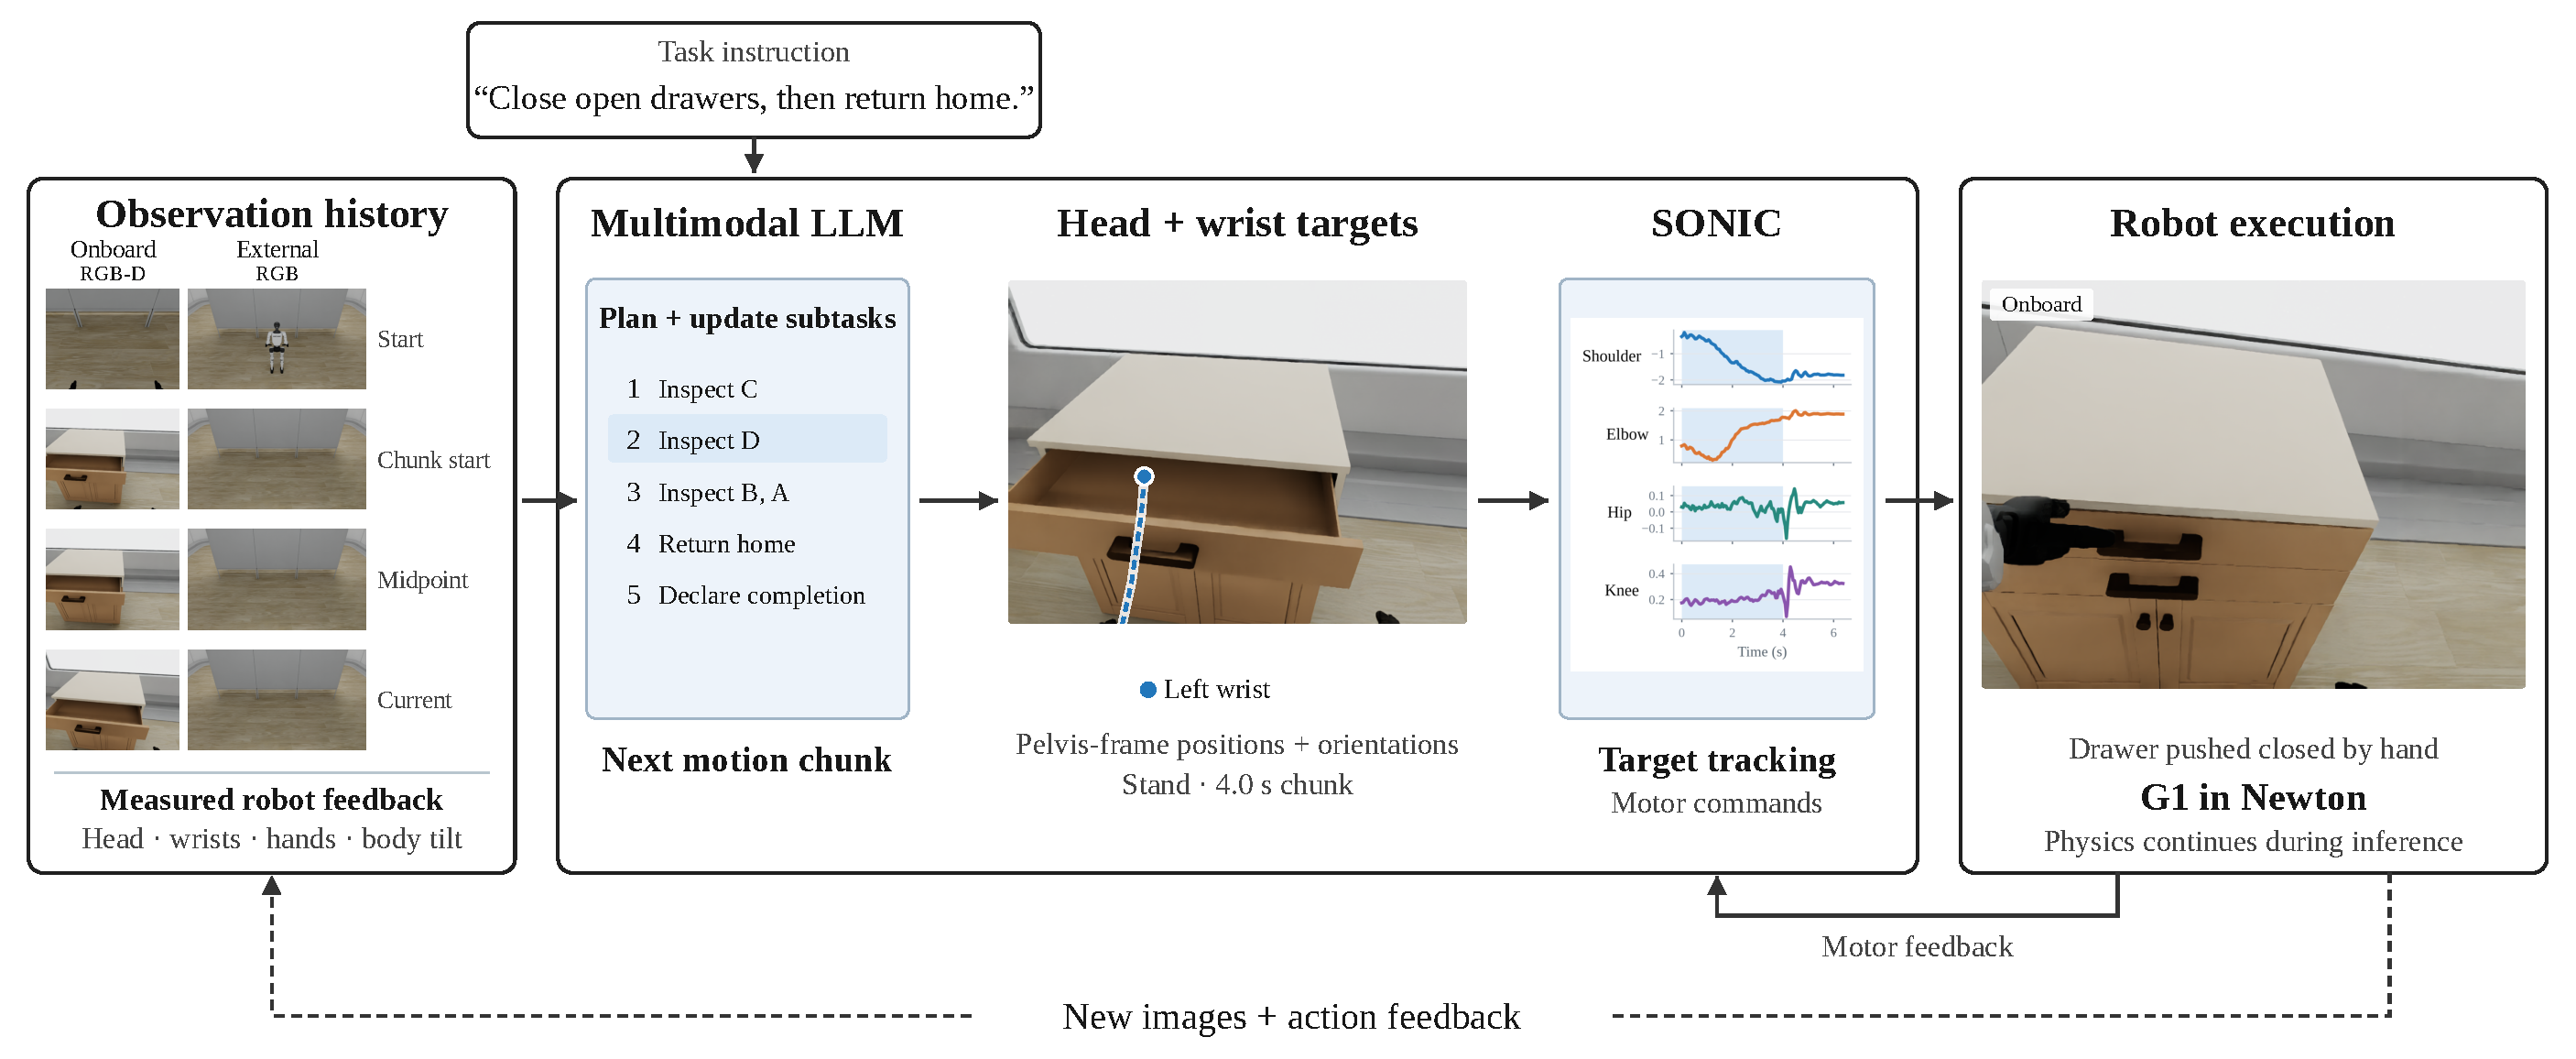
\includegraphics[width=\linewidth]{../docs/figures/system-overview.pdf}
  \par\smallskip
  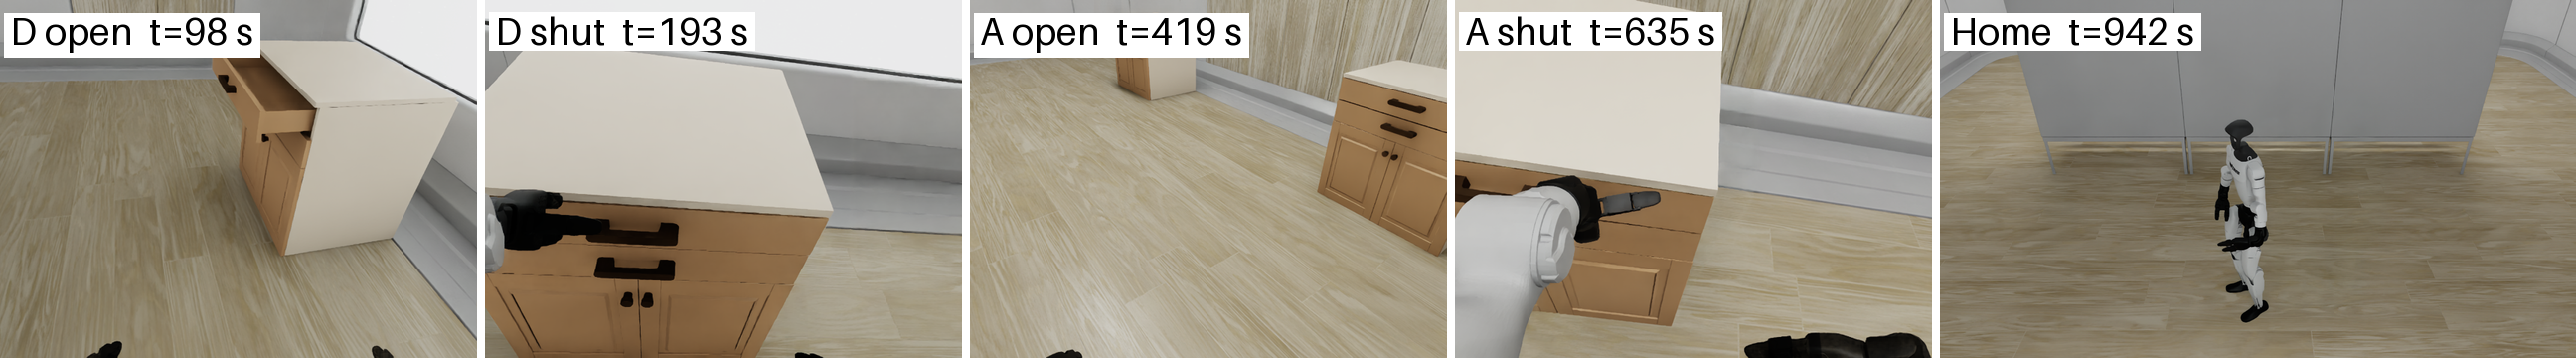
\includegraphics[width=\linewidth]{figures/astra-episode-sequence.png}
  \caption{Agent loop and original observations from a successful Astra low
  episode with A and D open. Home observation: 942\,s; declaration: 955\,s.}
  \label{fig:overview}
\end{figure}

\section{Online humanoid operation}
Room-scale humanoid operation couples navigation, inspection, contact and
stopping while physics continues during inference. We test frontier models'
ability to operate a humanoid through numerical references to the fixed SONIC
controller~\citep{sonic2026}. Prior work spans
skills~\citep{saycan2022,homebody2026,promptplanperform2024},
code~\citep{codeaspolicies2022,choi2026hugo},
visual feedback~\citep{innermonologue2022,pivot2024},
spatial representations~\citep{voxposer2023,sayplan2023,rekep2025}
and learned action representations~\citep{rt22023}.
Our approach uses numerical commands without predefined task skills,
generated policy code, value maps or keypoint constraints.

\section{Interface, task and evaluation}
\textbf{Interface.} Inputs are onboard RGB-D, external RGB, robot kinematics,
depth queries, a map, the plan and feedback (Fig.~\ref{fig:overview}). SONIC's
gamepad commands set walking speed, direction, facing and posture; three-point
tracking follows head/wrist positions and orientations. Four pose keyframes
span a chosen duration; hand presets are optional. Drawer states,
contacts and scores are withheld.

\textbf{Task.} Inspect four top drawers, push open ones shut by hand, leave
closed ones undisturbed, return home and declare completion. Four passive Sektion
drawers~\citep{isaaclab2026cabinet} occupy Simple
Room~\citep{nvidia2026warehouseassets,nvidia2026assetlicense}: A/B behind
lockers~\citep{nvidia2026simready}, C/D behind home; all fronts are initially hidden.
Eight initializations: none (control), A, B, C, D, A+B, A+D or B+C open;
all open drawers start at 0.20\,m under the same instruction. Newton~\citep{newton2025}
in Isaac Lab~\citep{isaaclab2025} runs at 200\,Hz.

\textbf{Evaluation.} Success requires all drawers within 2\,cm of shut at
$\leq$1\,cm/s for 1\,s, a supported standing hold within 25\,cm of home and a
completion declaration. Inspection, hand attribution and disturbance are scored
separately. After pilots, we froze the setup and 1800\,s budget. GPT-6 Astra,
GPT-6.1 Sol, Claude Opus 5.5 and Gemini 4 Argon ran once per condition/effort,
four concurrently.

\section{Results}
\begin{table}[htbp]
  \centering
  \small
  \setlength{\tabcolsep}{3pt}
  \begin{tabular}{lccccccc}
    \toprule
    Model / effort & Success & \shortstack{Physical\\completion} &
    \shortstack{False\\declarations} & Falls &
    \shortstack{Mean API\\cost (\$)} & \shortstack{Episode\\time (s)} & \shortstack{Decision\\latency (s)} \\
    \midrule
    Astra / low & 6/7 & 6/7 & 0/7 & 1/7 & 9.30 / 10.57 & 817 / 926 & 9.2 \\
    Astra / high & 6/7 & 6/7 & 0/7 & 1/7 & 7.65 / 8.78 & 998 / 1145 & 21.4 \\
    Sol / low & 4/7 & 4/7 & 1/7 & 2/7 & 1.72 / 1.96 & 829 / 940 & 10.4 \\
    Sol / high & 3/7 & 5/7 & 0/7 & 2/7 & 1.74 / 1.59 & 1235 / 1162 & 21.5 \\
    Opus / low & 2/7 & 3/7 & 2/7 & 3/7 & 4.78 / 6.23 & 762 / 1028 & 13.2 \\
    Opus / high & 3/7 & 3/7 & 1/7 & 2/7 & 7.22 / 8.36 & 1392 / 1563 & 36.1 \\
    Gemini / low & 0/7 & 0/4 & 0/4 & 3/4 & 1.29$^{*}$ / -- & 737 / -- & 32.3 \\
    Gemini / high & 0/7 & 0/5 & 0/5 & 1/5 & 1.59$^{*}$ / -- & 1332 / -- & 136.7 \\
    \bottomrule
  \end{tabular}
  \caption{Seven scheduled task attempts per row. Physical completion: goal reached
  at least once; false declarations: goal unmet when claimed. API errors remain
  in success denominators only. Gemini: three low-effort filter rejections,
  two high-effort timeouts.
  Cost/time: all/successful means through termination. Costs: usage at published
  rates~\citep{openai2026pricing,anthropic2026pricing,google2026pricing};
  GPU costs excluded; $^{*}$ excludes unresolved usage; --: no success.
  Latency: median of per-attempt medians for completed decisions.}
  \label{tab:results}
\end{table}
\textbf{Performance.} Astra led (6/7 each); 11/12 successes viewed all four drawer
fronts. Sol followed with 7/14 successes, Opus with 5/14, and Gemini with none
(Table~\ref{tab:results}). All 43 closures were by hand; no initially closed drawer
was disturbed.

\textbf{High vs.\ low effort.} Higher effort increased decision latency roughly
$2$--$4\times$; Astra's success was unchanged and Opus improved. Sol high closed
more open drawers (9/10 vs.\ 4/10) and physically completed more tasks (5/7 vs.\ 4/7),
but two went unreported before timeout or fall, yielding fewer successes
(3/7 vs.\ 4/7). Another Sol high run fell before any model command.

\textbf{Falls.} Of eight all-closed controls, three succeeded, four fell and one
had an API error. Overall, 16/19 falls lacked recorded drawer contact; other
collisions remain possible. Eleven of 18 post-command falls ended in holds
commanding zero translational speed with retained pose/facing targets. We hypothesize that prolonged target holds
during inference contribute to instability.

\textbf{Cost.} Astra high matched low's success at 18\% lower mean API cost; cached reads
covered 50\% of input versus 29\% at low, despite more output tokens.
Successful runs cost less for Sol high (\$1.59 vs.\ \$1.96), but including failures,
Sol low spent less per success (\$3.00 vs.\ \$4.06).

\textbf{Limitations.} One layout and one trial per model/effort/condition limit
generalization; 41/58 completed episodes exceeded 100\,ms peak physics lag.
Reliability and transfer need repeated trials and hardware tests.

\clearpage
\bibliography{../docs/references}
\end{document}
